\section{Analisi delle caratteristiche del dataset}
In questa fase preliminare si analizzano le principali caratteristiche statistiche delle variabili, al fine di comprendere la struttura dei dati e individuare eventuali anomalie.

\subsection{Analisi grafica tramite boxplot}
Di seguito si riportano i boxplot relativi alla variabile dipendente e alle variabili indipendenti.

\begin{figure}[H]
	\centering
	\subfigure[Boxplot della variabile dipendente \texttt{y\_VideoQuality}]{
		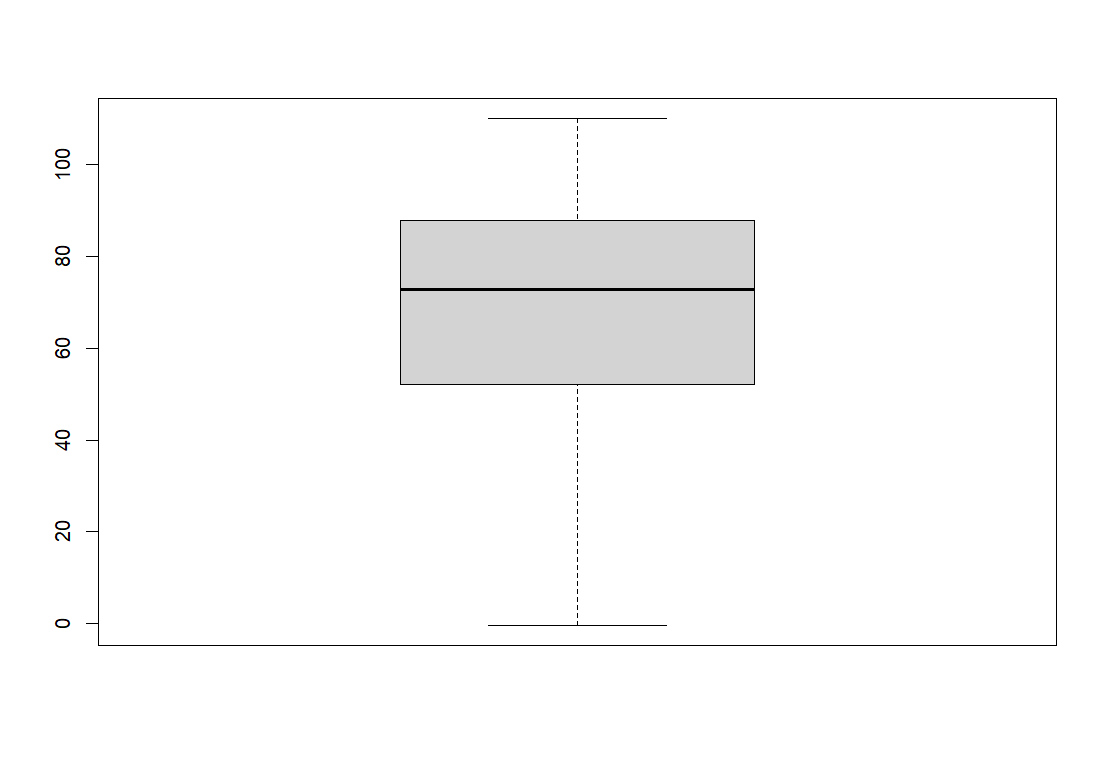
\includegraphics[width=0.65\linewidth]{graphs/DescriptiveStatisticPlots/boxplot_y_VideoQuality}
		\label{fig:boxplot_y_videoquality}
	}
	
	\vspace{1em} % spazio verticale tra le due sottofigure
	
	\subfigure[Boxplot delle variabili indipendenti \texttt{x\_i}]{
		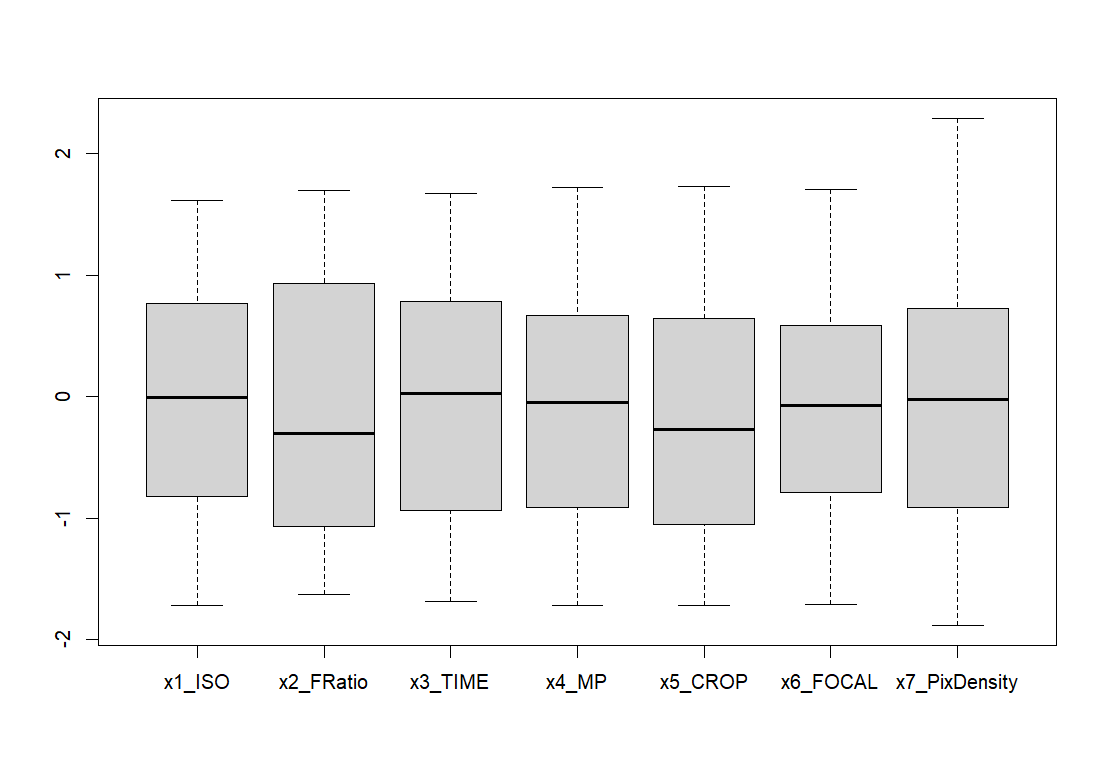
\includegraphics[width=0.65\linewidth]{graphs/DescriptiveStatisticPlots/boxplot_all_x_i}
		\label{fig:boxplot_all_xi}
	}
	\caption{Boxplot delle variabili considerate}
	\label{fig:boxplot_variabili}
\end{figure}


Dai grafici si osserva che tutti i valori di ciascuna variabile rientrano nei loro range interquartili, dunque non si evidenziano valori anomali (outlier).  
Per la variabile dipendente \texttt{y\_VideoQuality}, media e mediana risultano essere pari a: 
\[
\text{media} = 72.8135, \quad \text{mediana} = 68.6081,
\]
  
Si nota inoltre che la variabile \texttt{x7\_PixDensity} mostra una variabilità maggiore rispetto agli altri regressori, coprendo un intervallo maggiore rispetto alle altre variabili indipendenti.

\subsection{Verifica della normalità}
Sebbene la normalità delle variabili indipendenti non sia strettamente necessaria per la regressione lineare, si è comunque verificata graficamente e analiticamente la loro distribuzione.

\begin{figure}[H]
	\centering
	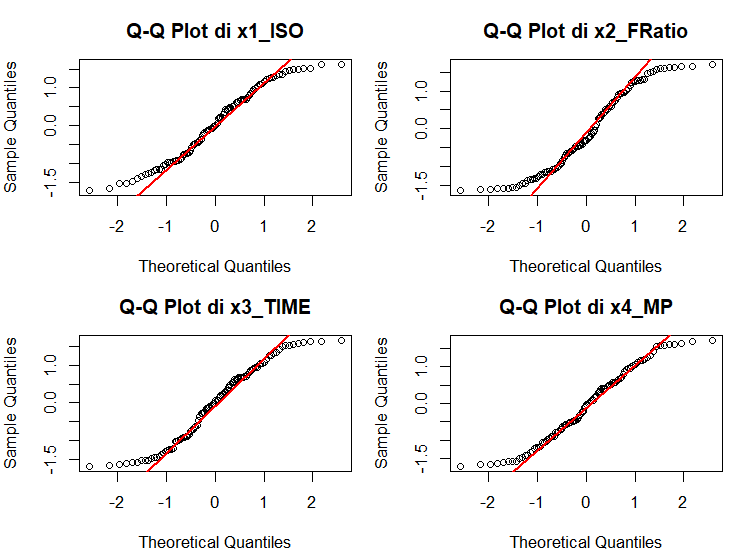
\includegraphics[width=0.9\linewidth]{graphs/DescriptiveStatisticPlots/qqplot1/qqplot1}
	\label{fig:qqplot1}
\end{figure}

Tra i diversi Q-Q plot analizzati, la variabile \texttt{x6\_FOCAL} mostra una forma visivamente compatibile con una distribuzione normale. Tuttavia, il test di Shapiro–Wilk applicato alla stessa fornisce i seguenti risultati:

\[
W = 0.97, \quad \text{p-value} = 0.02.
\]

Il valore di p-value ottenuto non si discosta molto da 0.05 e si potrebbe perciò supporre che la variabile sia distribuita come una normale.

\begin{figure}[H]
	\centering
	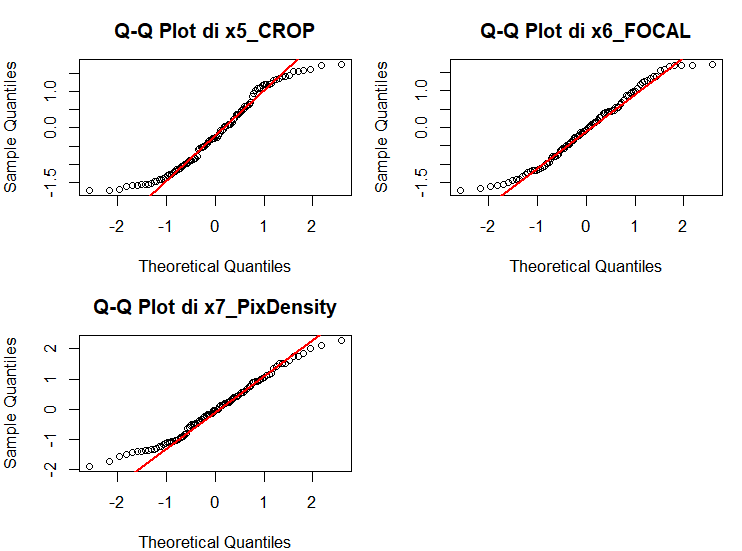
\includegraphics[width=0.9\linewidth]{graphs/DescriptiveStatisticPlots/qqplot1/qqplot2}
	\label{fig:qqplot2}
\end{figure}

